%% 
%% Copyright 2007-2024 Elsevier Ltd
%% 
%% This file is part of the 'Elsarticle Bundle'.
%% ---------------------------------------------
%% 
%% It may be distributed under the conditions of the LaTeX Project Public
%% License, either version 1.3 of this license or (at your option) any
%% later version.  The latest version of this license is in
%%    http://www.latex-project.org/lppl.txt
%% and version 1.3 or later is part of all distributions of LaTeX
%% version 1999/12/01 or later.
%% 
%% The list of all files belonging to the 'Elsarticle Bundle' is
%% given in the file `manifest.txt'.
%% 
%% Template article for Elsevier's document class `elsarticle'
%% with harvard style bibliographic references

\documentclass[preprint,12pt]{elsarticle}

%% Use the option review to obtain double line spacing
%% \documentclass[preprint,review,12pt]{elsarticle}

%% Use the options 1p,twocolumn; 3p; 3p,twocolumn; 5p; or 5p,twocolumn
%% for a journal layout:
%% \documentclass[final,1p,times]{elsarticle}
%% \documentclass[final,1p,times,twocolumn]{elsarticle}
%% \documentclass[final,3p,times]{elsarticle}
%% \documentclass[final,3p,times,twocolumn]{elsarticle}
%% \documentclass[final,5p,times]{elsarticle}
%% \documentclass[final,5p,times,twocolumn]{elsarticle}

%% For including figures, graphicx.sty has been loaded in
%% elsarticle.cls. If you prefer to use the old commands
%% please give \usepackage{epsfig}

%% The amssymb package provides various useful mathematical symbols
\usepackage{amssymb}
%% The amsmath package provides various useful equation environments.
\usepackage{amsmath}
%% The amsthm package provides extended theorem environments
%% \usepackage{amsthm}

%% The lineno packages adds line numbers. Start line numbering with
%% \begin{linenumbers}, end it with \end{linenumbers}. Or switch it on
%% for the whole article with \linenumbers.
%% \usepackage{lineno}

%\usepackage[utf8]{inputenc}
%\usepackage[T1]{fontenc}
\usepackage{gensymb}
\usepackage{algorithm}
\usepackage{algorithmic}
\usepackage{multirow}
\usepackage{xcolor}
\usepackage{colortbl}

\journal{Mathematics and Computers in Simulation}

\begin{document}

\begin{frontmatter}

%% Title, authors and addresses

%% use the tnoteref command within \title for footnotes;
%% use the tnotetext command for theassociated footnote;
%% use the fnref command within \author or \affiliation for footnotes;
%% use the fntext command for theassociated footnote;
%% use the corref command within \author for corresponding author footnotes;
%% use the cortext command for theassociated footnote;
%% use the ead command for the email address,
%% and the form \ead[url] for the home page:
%% \title{Title\tnoteref{label1}}
%% \tnotetext[label1]{}
%% \author{Name\corref{cor1}\fnref{label2}}
%% \ead{email address}
%% \ead[url]{home page}
%% \fntext[label2]{}
%% \cortext[cor1]{}
%% \affiliation{organization={},
%%             addressline={},
%%             city={},
%%             postcode={},
%%             state={},
%%             country={}}
%% \fntext[label3]{}

\title{Inflection Points for Similar Trajectory Retrieval} %% Article title

%% use optional labels to link authors explicitly to addresses:
%% \author[label1,label2]{}
%% \affiliation[label1]{organization={},
%%             addressline={},
%%             city={},
%%             postcode={},
%%             state={},
%%             country={}}
%%
%% \affiliation[label2]{organization={},
%%             addressline={},
%%             city={},
%%             postcode={},
%%             state={},
%%             country={}}
%AUTHOR 1
\author[1,2]{Lucija \v{Z}u\v{z}i\'{c}}
\ead{lucija.zuzic@uniri.hr}

\author[1,2]{Franko Hr\v{z}i\'{c}}
\ead{franko.hrzic@riteh.uniri.hr}

\author[2,3]{Irena Petrijev\v{c}anin}
\ead{ipetrijevcanin@mup.hr}

\author[1,2]{Jonatan Lerga\corref{cor1}}%\fnref[label2]
\ead{jonatan.lerga@riteh.uniri.hr}
 
% Address/affiliation
\affiliation[1]{organization={Department of Computer Engineering, Faculty of Engineering, University of Rijeka},
addressline={Vukovarska 58}, 
%         city={Rijeka},
%citysep={Rijeka}, % Uncomment if no comma needed between city and postcode
postcode={51000 Rijeka}, 
country={Croatia}}

\affiliation[2]{organization={Center for Artificial Intelligence and Cybersecurity, University of Rijeka},
addressline={Radmile Matejcic 2}, 
postcode={51000 Rijeka}, 
country={Croatia}}

\affiliation[3]{organization={Ministry of the Interior of the Republic of Croatia},
addressline={Ulica grada Vukovara 33}, 
postcode={10000 Zagreb}, 
country={Croatia}}

%\fntext[label2]{http://www.riteh.uniri.hr/osoba/jonatan-lerga}
% Corresponding author text
\cortext[cor1]{Corresponding author} 

%% Abstract
\begin{abstract}
Recognizing potentially reckless and inexperienced drivers of personal watercraft, especially those renting them, is imperative to avoid collisions and hazards, especially in crowded spaces during the peak of the tourist season. One potential way to recognize such drivers is by examining their driving patterns and trajectories that arise from them. A trajectory consists of points in a two-dimensional coordinate system, obtained from GPS (Global Positioning System) transmissions and paired with timestamps, representing the path traversed by a vehicle in a given ride. Separating drivers based on the trajectories is a demanding challenge due to the difference in trajectory patterns, lengths, and versatility of environments where rides occur. In this study, a novel algorithm based on inflection points of the trajectories is used to cluster similar trajectories and, thereby, drivers' behavior. The study aims to investigate and properly evaluate the clustering capabilities of Density-Based Spatial Clustering Applications with Noise (DBSCAN) and K-means when using features based on inflection points that represent the trajectory. Comprehensively evaluation is done by conducting a large-scale experiment with human raters and comparing the results to the generated clustering, indirectly evaluating the proposed algorithm for extracting inflection points from the trajectories.
\end{abstract}

%%Graphical abstract
%\begin{graphicalabstract}
%\includegraphics{grabs}
%\end{graphicalabstract}

%%Research highlights
%\begin{highlights}
%\item A novel trajectory segment classification metric using inflection point sequences
%\item Retrieving an entire trajectory and measuring the similarity to another sample
%\item Additionally detecting anomalies based on the smallest cluster
%\item Large-scale human evaluation using a web application to validate clustering
%\end{highlights}

%% Keywords
\begin{keyword}
personal watercraft \sep trajectory \sep classification \sep clustering
\end{keyword}

\end{frontmatter}

%% Add \usepackage{lineno} before \begin{document} and uncomment 
%% following line to enable line numbers
%% \linenumbers

%% main text
%%

% MAIN TEXT 
\section{Introduction}
 
When driving personal vehicles, on land or water, it is desirable to limit the possibility of human error and thereby prevent accidents. For this reason, some facilities for personal watercraft rental have installed a tracking system on their vehicles, such as the OtoTrak system \cite{ototrakOtoTrakTrack}, which provided database access for this study. The limits of the permitted driving zone in the studied system \cite{ototrakOtoTrakTrack} are determined according to latitude and longitude. Global Positioning System (GPS) signals enable all system features \cite{ototrakOtoTrakTrack} by periodically emitting records to be included in the database. Speed limits have been implemented once a driver ventures outside the zone or in the proximity of another vehicle with the same cloud-based marine watercraft tracking system that includes vehicle remote control. This study proposes an algorithm to detect anomalies that could replace this hard-coded system.
 
Anomalies in maritime traffic may be associated with various incidents, including criminal activities such as smuggling or illegal transshipment, as well as accidents like navigation failure or engine damage. The excess data from different information systems and sensors can be difficult to process \citep{2013Kazemi}, so efficient anomaly detection algorithms are critically important.

Examples of maritime anomalies include vessels that move randomly in open water, stop suddenly before reaching their destination, travel very short distances, encounter many other vessels, have a high frequency of looping, appear to cross land according to transmitted data, deviate from planned routes, exceed the speed limit, violate traffic regulations and so on \citep{2014Mascaro, 2008Laxhammar}.

Chandola et al. \citep{2009Chandola} provide a different definition of vessel behavior abnormalities than Martineau and Roy \citep{2011Martineau}, proving that a consensus has not been reached on this topic. The term anomaly has multiple connotations across domains, making it a somewhat vague idea with different interpretations among domain experts \citep{2008Roy}. In many data-rich areas, such as global maritime trade \citep{2022Kim}, most historical data are assumed to be normal. The anomaly detection algorithm initially considers any deviation from the models created based on such data an anomaly.

This work aims to classify driver behavior based on the inflection points of the trajectory of a personal watercraft represented by a function. The standard mathematical definition of an inflection point in two dimensions is used, meaning the movement direction on either axis changes. Each inflection point is assigned a type based on whether the $x$ and $y$ coordinates increase or decrease before and after the inflection point. Inflection points in our work are identified on subsets of a trajectory of ten or twenty consecutive data points.

The most common sequences of types of inflection points represent the trajectory fingerprint. The trajectory fingerprints are used to classify the entire trajectory and cluster trajectories using K-means and Density-Based Spatial Clustering Applications with Noise (DBSCAN). Trajectories in the smallest cluster are marked as anomalies in this paper. An experiment where humans select the five most similar out of twenty possible trajectories is used to validate the algorithm. The classification generated in this paper can replace hard-coded systems and avoid unnecessary speed limits in situations that are not dangerous. Additionally, it guarantees the safety of the driver and other participants in maritime traffic.
 
No examples of classifying or measuring the similarity of personal watercraft trajectories were found in the literature reviewed. However, Dynamic Time Warping (DTW) has been utilized for assessing the similarity of trajectories \cite{2017Fu, 2021Pedroche} of other vehicles, both on land and at sea. A novel metric based on trajectory subsequences and inflection points is proposed in this paper, reducing the high computational cost of DTW. This makes the algorithm applicable for real-time routing problems involving multiple vehicles \cite{BERTAZZI2025104892}. Maritime vessels could also be automated using a mechanism akin to Adaptive Cruise Control (ACC) for land vehicles \cite{YU2025104931, GUAN2025104914}, even in lane-free traffic \cite{BEZA2025104898}, so this work is highly relevant for watercraft fleets.

Many studies on trajectory tracking control use Lyapunov’s direct method for inertia matrix decomposition and the Lipschitz representation for the nonlinear longitudinal model of the vehicle. The vehicles used include underwater or horizontally moving vehicles, indoor airships, and wheeled robots. Boukhari et al. \cite{BOUKHARI2019236} proposed two Fault Tolerant Control (FTC) schemes for more reliable spacing control of an autonomous vehicle using the desired velocity in an Automated Highway System (AHS). Herman \cite{HERMAN20102317} uses a modified PD (proportional-derivative) controller for Autonomous Underwater Vehicles (AUVs). The application is expanded to different classes of vehicles in an experiment by Herman and Adamski \cite{HERMAN2020175}. Fu and Peng \cite{FU20231} use an adaptive iterative learning control strategy based on point-to-point trajectory update tracking for an Unmanned Aerial Vehicle (UAV) formation system. Xu et al. \cite{XU2022603} implement path planning for a wheeled robot using a different approach based on the inverse trajectory and the Martingale method since disturbances considered in other research are concerned with the controllers or actuators, not the locating sensors. However, none of these approaches deal with personal watercraft trajectories. The competing methods are much more complex models, tailored to specific devices. The simple inflection point-based approach proposed in this study can be applied to any trajectory. The main contributions of this study are:

\begin{itemize}
    \item A novel trajectory segment classification metric using inflection point sequences
    \item Retrieving an entire trajectory and measuring the similarity to another sample
    \item Additionally detecting anomalies based on the smallest cluster
    \item Large-scale human evaluation using a web application to validate clustering
\end{itemize}

The rest of the paper is organized as follows. Other relevant work that detects anomalies in maritime traffic are listed in section \ref{sec:Related}. The dataset is described in section \ref{sec:Dataset}, followed by the methodology used in this paper outlined in section \ref{sec:Methodology}. The results are discussed in section \ref{sec:Results}. Next, the main points are summarised, and the conclusion is given in section \ref{sec:Conclusion}.

\section{Related Work}
\label{sec:Related}

Since the goal was to classify trajectories, various papers on trajectories of larger vehicles were studied due to a scarcity of work on personal watercraft trajectories. The most commonly utilized approaches for this purpose are DBSCAN and K-means, while the K-means algorithm is used far less frequently than DBSCAN. 

One notable example is a study by Hanyang et al. \citep{2019Hanyang} using K-means on Automated Identification System (AIS) data from the National University of Defense Technology's "TianTuo-3" satellite. They identify the number of clusters using the elbow rule. The clustering features are the normalized standard deviation of the course over ground and speed over ground of South African vessels. Unlikely behavior is identified as an anomaly regarding a vessel's sailing stability.

DBSCAN can have several advantages over K-means. Namely, DBSCAN clusters do not have a fixed size and shape because they are based on density. Density-based clusters are useful for marine data, which is highly dense in some areas and sparse in others. On the other hand, K-means does not perform as well with unevenly distributed data or without clearly defined groups. Hence, DBSCAN overcomes these obstacles and is suited for varying shapes and densities of data distributions since the number of clusters is not predefined.

As mentioned before, maritime monitoring using AIS datasets often utilizes DBSCAN because it can detect noise and delete extraneous marine objects \citep{2018Coscia, 2018dAfflisio1, Ester1996ADA, Khan2004RealtimePO}. Unlike DBSCAN, K-means underperforms in the presence of outliers and noise.

DBSCAN clustering varies greatly with the input parameters. These parameter modifications can be challenging and time-consuming. The K-means algorithm has fewer parameters to tune, the most important being the number of clusters. DBSCAN results are usually highly accurate with properly defined parameters such as the number of points and maximum distance of points in a cluster. The resulting clusters are more flexible than K-means which has a fixed number of cluster centroids and splits the data according to distance from these points without considering distribution density.

Table~\ref{tab:DBSCANdetect} demonstrates that density-based spatial clustering techniques, especially DBSCAN \citep{Ester1996ADA}, are widely used in detecting abnormal vessel behavior. As the other algorithms in Table~\ref{tab:DBSCANdetect} illustrate, DBSCAN is usually not a standalone method, requiring a probability density distribution and a distance metric, and is often the input for additional processing steps.

Dynamic Time Warping (DWT) is often used for assessing the similarity of trajectories \cite{2017Fu, 2021Pedroche} but has a high computational cost for longer trajectories. The algorithm developed and proposed in this paper does not require the time-consuming and computationally intensive step of time-series alignment done in DTW. This novel approach separates the trajectory into subsequences and detects inflection points instead.

The most recent study referenced in this section \cite{2023Li} uses Long Short-Term Memory (LSTM), following trends in the development and wider use of deep learning. This study is not focused on a similar approach since embedded systems often do not meet the hardware requirements for implementing Recurrent Neural Networks (RNN), and real-time systems require fast responses.

Other models use information on position, speed, and course \cite{2014Wang, 2015Pallotta, 2018Lei, 2023Li}, while the proposed algorithm uses only position. This decision was made assuming that personal watercraft change speed and course more often because they have stronger engines and smaller dimensions than maritime vessels studied in related work. For this reason, any limits proposed for speed and course might be too strict to detect anomalies. Sudden turns can also be detected in location data forming a trajectory mitigating concerns about loss of information.

The referenced models are trained and tested on real AIS datasets \cite{2023Li, 2015Pallotta, 2017Fu} that are abundant and easily accessible. On the other hand, the developed models focus on a specific area, such as data gathered near Brest by the Naval Academy Research Lab \cite{2013Pallotta2} or the Chinese QiongZhou strait \cite{2018Lei}, meaning the model is only valid for a specific use case. However, the proposed algorithm is not location-specific and processes data from multiple locations worldwide, providing higher usability and transferability without relying on route extraction.

Note that DBSCAN clusters in many related papers use critical points of AIS tracks to create waypoints where vessels stop, enter, or exit the region of interest. Using these waypoints as nodes, graphs where maritime routes represent edges are created. Clustering methods relying on graphs will not always be able to connect a track to an edge of the normality graph, which hinders the possibility of assigning a track's start and end points to any waypoint. These methods apply only to cargo and tanker vessels or other vessel types that follow predetermined traffic route patterns. Fishing vessels and many others do not conform to these rules. Preprocessing is necessary for an operational system to separate different vessel types, as AIS metadata is often inaccurate.

Some methods, like the proposed algorithm in this study, use complete trajectories to detect anomalies or group trajectories based on similarity metrics \citep{2011Laxhammar, Vries2013}. Liu et al. \citep{2015Liu} debated an "ad-hoc" similarity measure for creating and grouping trajectory segments. Since DBSCAN is usually restricted to point clustering, this method can be explained as DBSCAN applied to trajectory clustering. 

Not all clustering methods rely on graphs but use a single point instead \citep{2012Kowalska, 2013Guillarme}. Grid cell size can lower the effectiveness of point-based methods for marine traffic analysis because they use the number of AIS messages in each cell. If a cell is too large, the prediction accuracy is lowered. A reliable local statistical model cannot be created if the grid is divided into too many sections. For these reasons, point-based techniques can only be used in regions with a low AIS message density. Trajectory-based techniques do not depend on grids and are more resilient regarding message density. However, trajectory-based techniques need sufficiently dense sub-areas inside a region of interest to successfully cluster waypoints and create reliable piecewise linear approximations of trajectories.

\begin{table}[!ht]
    \centering
    \begin{tabular}{|c|c|c|c|c|}
        \hline
        Author & Year & Algorithm \\ \hline
        Pallotta & 2013 & DBSCAN, \\
        et al. \cite{2013Pallotta2} & & Kernel Density Estimation (KDE) \\ \hline
         & & Speed and Direction DBSCAN, \\
        Wang et al. \cite{2014Wang} & 2014 & the Parallel Meta-Learning (PML), \\
         & & algorithm on Hadoop \\ \hline
        Pallotta and & 2015 & DBSCAN, on/off route, \\
        Jousselme \cite{2015Pallotta} & & speed/heading anomaly on route \\ \hline
        Sun et al. \cite{2015Sun} & 2015 & DBSCAN, unsupervised, extract \\
         & & traffic patterns from time/location \\ \hline
         Li et al. \cite{Li2017ADR} & 2017 & DTW, spectral clustering, \\
         & & Principal Component Analysis (PCA) \\ \hline
        Fu et al. \cite{2017Fu} & 2017 & DBSCAN, abnormal trajectories, DTW, \\
         & & Piecewise Linear Segmentation (PLS) \\ \hline
         & & DBSCAN, extract gravity vectors, \\
        Lei and & 2018 & sample stop points from clusters, \\
        Mingchao \cite{2018Lei} & & cluster relative and angular distance, \\
         & & distance  and speed/heading anomaly \\ \hline
        Botts \cite{2021Botts} & 2021 & DBSCAN, asymptotic properties \\
         & & of a novel anomaly metric \\ \hline
        Pedroche et al. \cite{2021Pedroche} & 2021 & DBSCAN, DTW, data mining \\ \hline
         & & Course/Speed-DBSCAN, \\
        Li et al. \cite{2023Li} & 2023 & Long Short-Term Memory (LSTM), \\
         & & added geospatial features \\ \hline
    \end{tabular}
    \caption{Sources using DBSCAN and other algorithms to detect unusual vessel trajectories the position, speed, and course variables obtained from AIS data.}
    \label{tab:DBSCANdetect}
\end{table}

\section{Dataset}
\label{sec:Dataset}

The database \cite{ototrakOtoTrakTrack} contains information about the rental locations, the vehicles, and the data sent for each ride, including speed, heading, latitude, and longitude. In this paper, only the latitude, and longitude data were used to detect and prevent anomalies.

Vehicle trajectories were recorded in Croatia, Spain, Portugal, Greece, Canada, and the USA in July 2022 and 2023. Trajectories, where the maximum time between two records in the database was greater than or equal to five seconds, were disregarded since the expected time equals one second. Also, those trajectories marked as "ERROR" or "TRACKING" in the database were disregarded. The flag "ERROR" means that records are missing. In "TRACKING" mode, records are sent less often than usual, while the expected time between records is one second in normal operating modes.

The system \cite{ototrakOtoTrakTrack} identifies data of the same trajectory using unique location, vehicle, and ride numbers. This study processed data for $2171$ rides forming trajectories originating from $14$ locations and $19$ vehicles.

\subsection{Trajectory Preprocessing}

First, before inflection points are calculated, the trajectory must be entirely in the first Quadrant of a Cartesian coordinate system, have an ending $0$ $y$ coordinate, and starting $0$ $x$ and $y$ coordinates. A trajectory is first translated so that the starting point has a $0$ $x$ and $y$ coordinate. All coordinates are then transferred from a Cartesian to a polar coordinate system and rotated so that the final point lies on the $x$ axis and has a $0$ $y$ coordinate. If any part of the resulting trajectory lies on the negative part of the $x$ or $y$ axis, each coordinate in the corresponding axis is replaced by the distance from the maximum value of all the trajectory coordinates for the axis. The visual demonstration of trajectory preprocessing is displayed in Figure~\ref{fig:visual_transform}. The dash-dotted and light blue trajectory is unaltered, the dotted and orange trajectory is translated to a $0$ $x$ and $y$ starting coordinate and rotated, and the solid and green trajectory is mirrored to eliminate negative values. All points except the red diamonds that mark inflection points are dark blue circles.

\begin{figure}[!ht]
    \centering
    \includegraphics[width = 0.7 \linewidth]{rotate_illustrate_42.pdf}
    \caption{The visual demonstration of trajectory preprocessing. The original trajectory is dash-dotted and light blue. The dotted and orange trajectory is translated to a $0$ $x$ and $y$ starting coordinate and rotated to a $0$ $y$ ending coordinate. The mirrored trajectory to eliminate negative values is solid and green. The inflection points are red diamonds, and all other points are dark blue circles.}
    \label{fig:visual_transform}
\end{figure}

Two lists of similar trajectories exist because trajectories are separated into $10$ or $20$ points segments, as demonstrated in Figure~\ref{fig:splitting_new_demo}. The segments in this step overlap, but this does not result in duplicate entries because different surrounding points mean inflection points will not always be detected.

\begin{figure}[!ht]
    \centering
    \includegraphics[width = 0.99 \linewidth]{splitting_new12.pdf}
    \caption{An example of splitting a trajectory. The entire trajectory is solid and light blue. Window 1 is red, and points upward, while window 2 is green and points downward since they overlap. The start of window 1 is a red square. Window 1 with a window size of $10$ is a dash-dotted red line that ends with a wide red diamond. Window 1 with a window size of $20$ is a dotted red line that ends with a narrow red diamond. The start of window 2 is a green circle. Window 2 with a window size of $10$ is a dashed green line that ends with a triangle pointing right. Window 2 with a window size of $20$ is a solid green line that ends with a triangle pointing left.}
    \label{fig:splitting_new_demo}
\end{figure}

\subsection{Types of Inflection Points}

Inflection points occur when either the $x$ or $y$ coordinate stops increasing and starts decreasing, or vice versa. In this paper, each type of inflection point is represented by a hexadecimal, and binary code, as described in Table~\ref{tab:classes}. The visual demonstration for each inflection point type is displayed in Figure~\ref{fig:visual_class}.

The hexadecimal codes, where the first number equals the second, and the third equals the fourth, do not represent an inflection point. There are four such sequences, specifically $0$ ($0000$), $3$ ($0011$), $c$ ($1100$), and $f$ ($0011$). These codes are marked with a yellow background in Figure~\ref{fig:visual_class} and Table~\ref{tab:classes}. These sequences are used for movement in a constant direction. Using these codes, all trajectory segments are fully described, even where inflection points do not occur. 

In the binary value used to generate the hexadecimal code, the increase or decrease of the $x$ and $y$ coordinates before and after the inflection point is represented by $1$ or $0$. A sequence of inflection points describes each trajectory segment and a series of these segment descriptions will be called trajectory fingerprints in further text. Since trajectories have an unequal length, they are separated into $10$ or $20$ points segments. These segment sizes were chosen to allow multiple inflection points to occur in a segment while limiting the number of different sequences of inflection points. 

\begin{table}[!ht]
    \centering
    \begin{tabular}{|c|c|c|c|c|}
        \hline
        Hex & $x_{1}$ & $x_{2}$ & $y_{1}$ & $y_{2}$ \\ \hline
        \rowcolor{yellow} 0 & 0 & 0 & 0 & 0 \\ \hline
        1 & 0 & 0 & 0 & 1 \\ \hline
        2 & 0 & 0 & 1 & 0 \\ \hline
        \rowcolor{yellow} 3 & 0 & 0 & 1 & 1 \\ \hline
        4 & 0 & 1 & 0 & 0 \\ \hline 
        5 & 0 & 1 & 0 & 1 \\ \hline
        6 & 0 & 1 & 1 & 0 \\ \hline
        7 & 0 & 1 & 1 & 1 \\ \hline
        8 & 1 & 0 & 0 & 0 \\ \hline
        9 & 1 & 0 & 0 & 1 \\ \hline
        a & 1 & 0 & 1 & 0 \\ \hline
        b & 1 & 0 & 1 & 1 \\ \hline
        \rowcolor{yellow} c & 1 & 1 & 0 & 0 \\ \hline
        d & 1 & 1 & 0 & 1 \\ \hline
        e & 1 & 1 & 1 & 0 \\ \hline
        \rowcolor{yellow} f & 1 & 1 & 1 & 1 \\ \hline
    \end{tabular}
    \caption{The hexadecimal, and binary representation of the code for types of inflection points and the increase ($1$) or decrease ($0$) of the $x$ and $y$ coordinates before and after the inflection point.}
    \label{tab:classes}
\end{table}

\begin{figure}[!ht]
    \centering
    \includegraphics[width = 0.8 \linewidth]{class_illustrate_42.pdf}
    \caption{The visual demonstration for a hexadecimal, and binary representation of the code for types of inflection points and the increase ($1$) or decrease ($0$) of the $x$ and $y$ coordinates before and after the inflection point. The inflection point is a red diamond, the point before is a green triangle, and the point after is a dark blue circle.}
    \label{fig:visual_class}
\end{figure}

\subsection{Selecting Sequences of Inflection Points for Trajectory Fingerprints}

A total of $4678$ different sequences of inflection points occurred when separating trajectories into segments of $10$ points, and $31490$ different sequences of inflection points occurred when separating trajectories into segments of $20$ points. Only the frequency of the $200$ most frequent sequences of inflection points were used when calculating Euclidean distance and clustering trajectory fingerprints to decrease the complexity of the calculation and the memory requirements.

The total frequency of sequences of inflection points when separating trajectories into segments of either $10$ or $20$ points is visible in Table~\ref{tab:classes1020} with only sequences of inflection points with a frequency over $1\%$ being represented.

The displayed most frequent sequences of inflection points cover a larger portion of the trajectories when separating trajectories into segments of $10$ points, representing $91.24\%$ instead of $81.68\%$ of segments. The sequences of inflection points are longer and individually less frequent when separating trajectories into segments of $20$ points. This demonstrates a greater variety of sequences that a larger window size can distinguish.

The three most frequent sequences of inflection points when separating trajectories into segments of either $10$ or $20$ points are $e$, $ede$, and $ed$, previewed in Figure~\ref{fig:visual_class} and Table~\ref{tab:classes}. This demonstrates the similarity between both algorithms and the validity of using these sequences.

\begin{table}[!ht]
    \centering
    \begin{tabular}{|c|c|c|c|}
        \hline
        \multicolumn{2}{|c|}{Window size $10$} & \multicolumn{2}{c|}{Window size $20$} \\ \hline
        Sequence & Frequency & Sequence & Frequency \\ \hline
        e & $42.35\%$ & e & $21.99\%$ \\ \hline
        ede & $17.39\%$ & ede & $13.6\%$ \\ \hline
        ed & $16.32\%$ & ed & $9.68\%$ \\ \hline
        eded & $7.17\%$ & edede & $8.21\%$ \\ \hline
        edede & $4.46\%$ & eded & $7.47\%$ \\ \hline
        e8 & $2.26\%$ & ededed & $4.56\%$ \\ \hline
        ededed & $1.29\%$ & ededede & $4.01\%$ \\ \hline
        Total & $91.24\%$ & e8 & $3.9\%$ \\ \hline
        \multicolumn{2}{c|}{} & b2 & $3.49\%$ \\ \cline{3-4}
        \multicolumn{2}{c|}{} & edededed & $2.07\%$ \\ \cline{3-4}
        \multicolumn{2}{c|}{} & edededede & $1.47\%$ \\ \cline{3-4}
        \multicolumn{2}{c|}{} & e81 & $1.23\%$ \\ \cline{3-4}
        \multicolumn{2}{c|}{} & Total & $81.68\%$ \\ \cline{3-4}
    \end{tabular}
    \caption{The total frequency of sequences of inflection points with a frequency over $1\%$ when separating trajectories into segments of $10$ (left) or $20$ (right) points.}
    \label{tab:classes1020}
\end{table}

\section{Methodology}
\label{sec:Methodology}

\subsection{Design of a Human Similar Trajectory Selection Experiment}

Because ground truth classification in the dataset is unavailable, an experiment was conducted using a website inspired by Shanmugaraj et al. \citep{shanmugaraj2024smart} as a basis for validation and comparison with the algorithm. Due to time constraints, $28$ trajectories were used as a baseline in a similar trajectory selection experiment conducted with humans. A selection screen example is shown in Figure~\ref{fig:user_select}. Out of $20$ trajectories, users must select the $5$ most similar. The algorithm selects those with the smallest Euclidean distance of trajectory fingerprints. The order in which the $20$ trajectories are displayed is randomized.

\begin{figure}[!ht]
    \centering
    \includegraphics[width = 0.99 \linewidth]{Rate2.pdf}
    \caption{An example of the user selection screen for one testing condition. The baseline trajectory in the first row has a blue outline, the selected five trajectories have a green outline, and fifteen other trajectories have a red outline.}
    \label{fig:user_select}
\end{figure}

Two trajectories were randomly selected for each of the $14$ locations where personal watercraft are rented, as visible in Figure~\ref{fig:baseline}. An ordered list of all $2171$ trajectories is generated for each baseline trajectory, progressing from the smallest to the largest Euclidean distance of trajectory fingerprints. Two lists of similar trajectories exist because trajectories are separated into $10$ or $20$ points segments, as demonstrated in Figure~\ref{fig:splitting_new_demo}. The experiment is repeated for each user for each of the $28$ baseline trajectories split into $10$ or $20$ points segments, for a total of $56$ times per user.

\begin{figure}[!ht]
    \centering
    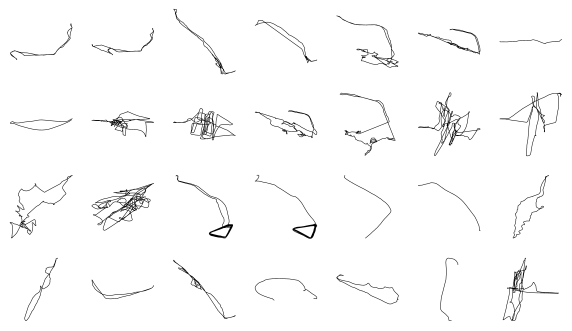
\includegraphics[width = 0.99 \linewidth]{baseline.pdf}
    \caption{The $28$ randomly selected baseline trajectories for the human selection experiment, two for each of the $14$ locations where personal watercraft are rented.}
    \label{fig:baseline}
\end{figure}

In the experiment, $20$ trajectories other than the baseline are displayed. These trajectories include the ones at the $1$st, $115$th, and all other places increasing by $114$ and less than $2171$, ending with the $2167$th place, based on the Euclidean distance of their fingerprints. The step size of $114$ was chosen because it divides the total number of $2171$ trajectories into $20$ equal parts with the smallest remainder.

The order in which the $56$ testing conditions are displayed for a user is determined by the class assigned to a user. A balanced Latin square is used to eliminate the order effect. An example of a balanced Latin square for four testing conditions represented by letters from $A$ to $D$ is given in Table~\ref{tab:latin}. Each row in the Latin square represents the order in which the testing conditions are displayed for a user assigned to the corresponding class. This ensures that an equal number of users see the testing conditions in a certain order. Users automatically get assigned to the class with the least participants when first registering. If multiple classes have the same number of participants, the class with the smallest number is chosen. In this analysis, $56$ users were included to ensure that each testing condition appears exactly once. This amounts to $1568$ conducted tests for subsequences of $10$ or $20$ points, for $56$ users and $28$ test trajectories.

\begin{table}[!ht]
    \centering
    \begin{tabular}{|c|c|c|c|}
        \hline
        A & B & C & D \\ \hline
        B & C & D & A \\ \hline
        C & D & A & B \\ \hline
        D & A & B & C \\ \hline
    \end{tabular}
    \caption{An example of a balanced Latin square for four testing conditions represented by letters from $A$ to $D$.}
    \label{tab:latin}
\end{table}

The experiment is designed to restrict navigation within a single testing condition, preventing the user from going back, moving forward, or changing a submitted answer. However, the entire experiment can be paused or repeated indefinitely, provided the browser tab remains open. If the experiment is repeated, any previously submitted answers are overwritten. If the user exits the experiment, they will need to restart from the beginning to resume participation.

\subsection{Clustering Trajectories Based on the Most Frequent Sequences of Inflection Points}

The trajectories were clustered using K-means and DBSCAN, based on the trajectory fingerprint when separating trajectories into segments of either $10$ or $20$ points. The DBSCAN and K-means algorithms were selected based on previous related work presented in section \ref{sec:Related}.

The DBSCAN algorithm used a fixed minimum number of $346$ points inside a cluster. This choice is based on research that indicates it should be larger than the number of features \cite{Ester1996ADA}, which in this case represent the $200$ most frequent sequences of inflection points used in a trajectory fingerprint. $346$ was the largest possible minimum number of points inside a cluster that produced at least two clusters to detect anomalies.

An $\epsilon$ parameter value of $6.086 \times 10^{-2}$ and $9.343 \times 10^{-2}$ was used for a window size of $10$ and $20$ respectively. The $\epsilon$ parameter value was determined by finding the elbow in a $k$-nearest neighbors plot of Euclidean distances based on trajectory fingerprints, as suggested by Rahmah and Sitanggang \cite{rahmah2016determination}. The $k$ value in a $k$-nearest neighbors plot was $346$, the same as the minimum number of points inside a cluster.

DBSCAN finds fewer and denser clusters if the minimum number of samples is larger, while K-means finds the specified number of clusters. The number of clusters DBSCAN generated was used for the K-means algorithm to allow comparisons. The trajectories in the smallest cluster DBSCAN or K-means are flagged as anomalies because it is assumed that most trajectories are normal.

To visualize the clusters of trajectories in two dimensions, the Principal Component Analysis (PCA) algorithm, with the number of components set to two, was applied to the trajectory fingerprint with multiple features when separating trajectories into segments of either $10$ or $20$ points. The PCA algorithm is chosen based on previous work that plots the data in two dimensions using the first two principal components to visually identify closely related data points in clusters \cite{jolliffe2016principal}.

\subsection{Comparing the Algorithm and Clustering with the User's Selection}

To assess how well an algorithm's selection aligns with the users, the five most similar trajectories selected by the user belong to the positive class. In contrast, the other fifteen out of twenty belong to the negative class. This means $25\%$ of samples belong to the positive, and $75\%$ to the negative class. The five trajectories the algorithm selected are classified into the positive class, while the other fifteen out of twenty are classified into the negative class.

Similarly, K-means and DBSCAN clustering for each window size are compared with the user's selection. The trajectories that belong to the same cluster as the baseline trajectory are classified into the positive class, and others belong to the negative class. The clustering can generate between $0$ and $20$ positive classifications, while the rest are negative. The arrays representing all users and trajectories are aligned with K-means and DBSCAN clustering results for each window size. In this way, each clustering algorithm is benchmarked against the users to see which classification method is more successful based on an independent ground truth value obtained from users.

A confusion matrix and the derived metrics can be used to assess the difference from the users' choices. The choices for all users and trajectories are merged in a single array for each window size since the window sizes use different algorithms. $1568$ tests are conducted for each window size, one for each combination of $56$ users and $28$ test trajectories. Thus, out of $31360$ samples, $20$ for each one among $1568$ tests, $7840$ samples belong to the positive class, $5$ for each test, and $23520$ to the negative class, $15$ for each test.

\subsubsection{Confusion Matrix}
%\label{subsubsec:ConfusionMatrix}

A correct classification is marked as a True Positive (TP), or True Negative (TN) result. A type I or II error in classification is marked as False Positive (FP) or False Negative (FN), respectively.

The percentage of correctly classified samples that truly belong to a class is evaluated by sensitivity, recall, hit rate, or True Positive Rate (TPR), calculated as $\mathrm{TP}/(\mathrm{TP}+\mathrm{FN})$, and specificity, selectivity, or True Negative Rate (TNR), calculated as $\mathrm{TN}/(\mathrm{TN}+\mathrm{FP})$ \cite{altman1994diagnostic1, altman1994diagnostic2}.

Precision, or Positive Predictive Value (PPV), calculated as $\mathrm{TP}/(\mathrm{TP}+\mathrm{FP})$, and Negative Predictive Value (NPV), calculated as $\mathrm{TN}/(\mathrm{TN}+\mathrm{FN})$, represent the ratio of correct assignment among samples classified to a class.

The proportion of samples of a class or classifications to a class is recorded by prevalence, calculated as $(\mathrm{TP}+\mathrm{FN})/(\mathrm{TP}+\mathrm{FP}+\mathrm{FN}+\mathrm{TN})$, and Detection Prevalence (DP), calculated as $(\mathrm{TP}+\mathrm{FP})/(\mathrm{TP}+\mathrm{FP}+\mathrm{FN}+\mathrm{TN})$, respectively. If prevalence is not equally distributed among classes, they are unbalanced.

The proportion of correct assignment for a single or any class is noted by the Detection Rate (DR), calculated as $\mathrm{TP}/(\mathrm{TP}+\mathrm{FP}+\mathrm{FN}+\mathrm{TN})$, and accuracy (Acc), calculated as $(\mathrm{TP} + \mathrm{TN}) / (\mathrm{TP} + \mathrm{TN} + \mathrm{FP} + \mathrm{FN})$, respectively.

Balanced Accuracy (BA) \cite{velez2007balanced} is used for unbalanced classes since accuracy does not consider them individually. In this study, there is only $25\%$ of positive samples. The formula $(\mathrm{TPR} + \mathrm{TNR}) / 2$ equals the arithmetic mean of TPR and TNR, focused on the positive and the negative classes, respectively.

Another metric that can be used instead of accuracy to consider each class separately is the $F1$ score, or the harmonic mean of PPV and TPR, calculated as $2 \times (\mathrm{PPV} \times \mathrm{TPR}) / (\mathrm{PPV} + \mathrm{TPR}) = 2 \times \mathrm{TP} / (2 \times \mathrm{TP} + \mathrm{FP} + \mathrm{FN})$.

\subsubsection{McNemar's test}
%\label{subsubsec:McNemar}

Created for techniques that distinguish between two classes, McNemar's test for correlated proportions is based on the chi-squared distribution and is applied to paired categorical data. Comparing the sensitivity and specificity of two candidate models directly is not as informative of model difference as the truth value of the null hypothesis of marginal homogeneity, which asserts that the marginal probability for each outcome is equal for both compared models \cite{mcnemar1947note}.

\section{Results and Discussion}
\label{sec:Results}
 
The clusters of trajectories generated by DBSCAN and K-means are illustrated in Figure~\ref{fig:10_20_DBSCAN_PCA} using two components generated by PCA of the trajectory fingerprint when separating trajectories into segments of $10$ or $20$ points. DBSCAN isolated a dense area surrounded by scattered data points, while K-means split the area into two equal surfaces regardless of density.

\begin{figure}[!ht]
    \centering
    \includegraphics[width = 0.99\linewidth]{DBSCAN_Kmeans_all_newn_2_PCA.pdf}
    \caption{DBSCAN and K-means clusters for a window size of $10$ or $20$ with two components generated by PCA of the trajectory fingerprint.}
    \label{fig:10_20_DBSCAN_PCA}
\end{figure}

Table~\ref{tab:DBSCAN_K-meansAnomalyEuclid} gives the average Euclidean distance of trajectory fingerprints in pairs where both, none, or only one is an anomaly for a window size of $10$ or $20$ and DBSCAN or K-means clusters.

\begin{table}[!ht]
    \centering
    \begin{tabular}{|c|c|c|c|c|} \hline
        Algorithm & Window size & Both & None & One \\ \hline
        K-means & $10$ & $0.1265$ & $0.2341$ & $0.1364$ \\ \hline
        K-means & $20$ & $0.1787$ & $0.1558$ & $0.2604$ \\ \hline
        DBSCAN & $10$ & $0.054$ & $0.1551$ & $0.1973$ \\ \hline
        DBSCAN & $20$ & $0.2795$ & $0.1382$ & $0.2494$ \\ \hline
    \end{tabular}
    \caption{The average Euclidean distance of trajectory fingerprints in pairs where both (left), none (center), or only one (right) is an anomaly for different window sizes and DBSCAN or K-means clusters.}
    \label{tab:DBSCAN_K-meansAnomalyEuclid}
\end{table}

The largest average Euclidean distance of trajectory fingerprints in pairs with different anomaly flags of $0.2604$ is achieved for K-means clusters and a window size of $20$. Pairs of two trajectories in different clusters have a larger average Euclidean distance of fingerprints than two trajectories with the same positive or negative anomaly flag for K-means clusters and a window size of $20$. This is not true for a window size of $10$ and K-means clusters, indicating that classified trajectories in one cluster are not well separated from others and are less similar to those inside their cluster.

For DBSCAN and a window size of $10$, pairs of two trajectories with the same anomaly flags have a smaller average Euclidean distance of fingerprints than two trajectories with different anomaly flags. This is not true for a window size of $20$ and DBSCAN clusters, indicating that normal trajectories are not well distinguished from anomalies and differ more significantly within the same cluster.

Table~\ref{tab:DBSCAN_K-meansAnomalySeq} shows the frequency of the $e$ sequence of inflection points among anomalous and non-anomalous trajectories for a window size of $10$ or $20$ and DBSCAN or K-means clusters. The $e$ sequence of inflection points, representing an increasing $x$ coordinate and a $y$ coordinate that first increases and then decreases, is shown here because it is the most frequent sequence of inflection points for both window sizes.

\begin{table}[!ht]
    \centering
    \begin{tabular}{|c|c|c|c|} \hline
        Algorithm & Window size & Anomalous & Non-anomalous \\ \hline
        K-means & $10$ & $50.77\%$ & $33.13\%$ \\ \hline
        K-means & $20$ & $33.76\%$ & $15.83\%$ \\ \hline
        DBSCAN & $10$ & $41.24\%$ & $41.99\%$ \\ \hline
        DBSCAN & $20$ & $25.39\%$ & $20.02\%$ \\ \hline
    \end{tabular}
    \caption{The frequency of the $e$ sequence of inflection points among anomalous (left) and non-anomalous (right) trajectories for different window sizes and DBSCAN or K-means clusters.}
    \label{tab:DBSCAN_K-meansAnomalySeq}
\end{table}

For a window size of $20$ and DBSCAN or K-means clusters, anomalous trajectories have a larger frequency of the $e$ sequence of inflection points than non-anomalous trajectories. For a window size of $10$, non-anomalous trajectories have a smaller frequency of the $e$ sequence of inflection points than non-anomalous trajectories only for the K-means, not the DBSCAN algorithm, even though the values $41.24\%$ and $41.99\%$ are very close. The frequency of the $e$ sequence of inflection points varies most significantly for a window size of $20$ and K-means clusters, dropping from $33.76\%$ to $15.83\%$ for non-anomalous trajectories, with a difference of $17.93\%$. These results support the conclusion that the $e$ sequence of inflection points indicates an anomaly and that a window size of $20$ and K-means clusters generate the best classification.

The confusion matrix performance indicators for window sizes of $10$ and $20$ and the algorithm without clustering, K-means, and DBSCAN are presented in Table~\ref{tab:DBSCAN_K-meansConfMatrix}.

\begin{table}[!ht]
    \centering
    \begin{tabular}{|c|c|c|c|c|c|c|} \hline
        Model & \multicolumn{2}{c|}{Algo vs. User} & \multicolumn{2}{c|}{K-means vs. User} & \multicolumn{2}{c|}{DBSCAN vs. User} \\ \hline
        Window size & $10$ & $20$ & $10$ & $20$ & $10$ & $20$ \\ \hline
        TP & $2704$ & $4397$ & $4431$ & $6115$ & $6017$ & $5360$ \\ \hline
        TN & $18384$ & $20077$ & $13223$ & $11659$ & $5569$ & $10960$ \\ \hline
        FP & $5136$ & $3443$ & $10297$ & $11861$ & $17951$ & $12560$ \\ \hline
        FN & $5136$ & $3443$ & $3409$ & $1725$ & $1823$ & $2480$ \\ \hline
        Sensitivity & $34.49$ & $56.08$ & $56.52$ & $78.0$ & $76.75$ & $68.37$ \\ \hline
        Specificity & $78.16$ & $85.36$ & $56.22$ & $49.57$ & $23.68$ & $46.6$ \\ \hline
        PPV & $34.49$ & $56.08$ & $30.09$ & $34.02$ & $25.1$ & $29.91$ \\ \hline
        NPV & $78.16$ & $85.36$ & $79.5$ & $87.11$ & $75.34$ & $81.55$ \\ \hline
        DR (P) & $8.62$ & $14.02$ & $14.13$ & $19.5$ & $19.19$ & $17.09$ \\ \hline
        DR (N) & $58.62$ & $64.02$ & $42.17$ & $37.18$ & $17.76$ & $34.95$ \\ \hline
        DP & $25.0$ & $25.0$ & $46.96$ & $57.32$ & $76.43$ & $57.14$ \\ \hline
        Acc & $67.24$ & $78.04$ & $56.29$ & $56.68$ & $36.95$ & $52.04$ \\ \hline
        BA & $56.33$ & $70.72$ & $56.37$ & $63.78$ & $50.21$ & $57.48$ \\ \hline
        F1 & $34.49$ & $56.08$ & $39.27$ & $47.37$ & $37.83$ & $41.61$ \\ \hline
    \end{tabular}
    \caption{The confusion matrix performance indicators for the algorithm without clustering (left), K-means (center), or DBSCAN (right) clusters compared to the user's selection. Results are separated for a window size of $10$ (left) and $20$ (right). All values except TP, TN, FP, and FN represent a percentage (\%).}
    \label{tab:DBSCAN_K-meansConfMatrix}
\end{table}

K-means, compared to user selection, has a larger specificity, PPV, NPV, accuracy, balanced accuracy, and F1 score than the DBSCAN algorithm for both window sizes. The DBSCAN algorithm has a larger sensitivity for a window size of $10$, but not for a window size of $20$. This means that K-means outperforms DBSCAN when aligned with user classification.

The algorithm without clustering compared to user selection has a larger specificity, PPV, NPV, accuracy, and balanced accuracy than the DBSCAN algorithm for both window sizes. The DBSCAN algorithm has a larger sensitivity and F1 score for a window size of $10$, but not for a window size of $20$. The results indicate that the DBSCAN algorithm is less similar to the user-selected values than the algorithm without clustering.

The algorithm without clustering compared to user selection has a larger specificity, PPV, and accuracy than the K-means algorithm for both window sizes. The K-means algorithm has a larger sensitivity and NPV for both window sizes, and a larger balanced accuracy and F1 score for a window size of $10$, but not for a window size of $20$. This means that K-means outperforms DBSCAN when aligned with user classification. The results indicate that the algorithm without clustering is more similar to user selection than the K-means algorithm.

K-means, DBSCAN, and the algorithm without clustering compared to user selection have a larger PPV, NPV, accuracy, balanced accuracy, and F1 score for a window size of $20$ than for a window size of $10$. This supports the conclusion that a larger window size enables better alignment with user's choices.

K-means compared, to user selection, has a larger specificity for a window size of $20$ than for a window size of $10$. DBSCAN has a larger sensitivity for a window size of $20$ when comparing window sizes. The algorithm without clustering has a smaller specificity and sensitivity for a window size of $10$ when comparing window sizes. This adds validity to the claim that a smaller window yields results dissimilar to user classification.

The marginal probabilities for both anomaly classes differ when comparing the algorithm without clustering and the user selection for both window sizes, since the $p$-values of McNemar's test equal $1$. The TP, TN, FP, and FN values from Table~\ref{tab:DBSCAN_K-meansConfMatrix} were used in the contingency tables for the statistical tests.  The $p$-values of McNemar's test equal $0$ when comparing either K-means, or DBSCAN clustering to user selection, so the null-hypothesis that marginal probabilities for both anomaly classes are equal cannot be rejected. This indicates that the algorithm without clustering is statistically significantly different from user selection, but this is not true after either clustering algorithm is applied.

\section{Conclusion}
\label{sec:Conclusion}

This work aims to classify driver behavior based on the inflection points of the function that represents the vehicle trajectory. Each inflection point is assigned a type based on whether the $x$ and $y$ coordinates increase or decrease before and after the inflection point. Inflection points are identified on subsets of a trajectory of $10$ or $20$ consecutive data points. The $200$ most common sequences of types of inflection points are used to generate a trajectory fingerprint, classify an entire trajectory, and cluster trajectories using K-means and DBSCAN. Anomalies are then identified as members of the smallest cluster. An experiment where humans select the five most similar out of twenty possible trajectories compared to a baseline trajectory is used to validate the algorithm by applying confusion matrix performance indicators. The algorithm without clustering compared to user selection has an accuracy of $78.04\%$ for a window size of $20$, supporting the hypothesis that an algorithm using inflection points matches human classification.

The average Euclidean distance of trajectory fingerprints is smaller for two anomalous or non-anomalous trajectories than for trajectories with different statuses for a window size of $20$ and K-means clusters. This validates the K-means algorithm with a larger window size. The $e$ sequence of inflection points is the most frequent one and represents an increasing $x$ coordinate and a shift from increasing to decreasing for the $y$ coordinate. For a window size of $20$ and K-means cluster, the frequency of the $e$ sequence of inflection points is larger for anomalies. These results further support the K-means algorithm and a window size of $20$.

DBSCAN, compared to user selection, has a lower specificity, PPV, NPV, accuracy, balanced accuracy, and F1 score than the K-means algorithm for both window sizes. This supports the conclusion that K-means clustering better matches user selection than DBSCAN.

The algorithm without clustering compared to user selection has a larger sensitivity, specificity, PPV, NPV, accuracy, balanced accuracy, and F1 score for a window size of $20$ than for a window size of $10$. This indicates that a window size of $10$ yields an algorithm different from user ratings, so a larger window size of $20$ might be beneficial. Future research may consider a larger window size on a larger dataset.

The algorithm without clustering is statistically significantly different from user selection according to the $p$-values of McNemar's test for either window size. This statement does not hold if K-means or DBSCAN clustering algorithm is used, making a case for the usefulness of the generated clustering.

% conflicts of interest
\section*{Declaration of competing interest}
The authors declare no conflict of interest.

\section*{CRediT authorship contribution statement}
\textbf{Lucija \v{Z}u\v{z}i\'{c}:} Conceptualization, Methodology, Software, Validation, Investigation, Data Curation, Writing -- Original Draft, Visualization. \textbf{Franko Hr\v{z}i\'{c}:} Conceptualization,  Validation, Formal analysis, Investigation, Resources, Writing -- Original Draft, Writing -- Review \& Editing, Supervision. \textbf{Jonatan Lerga:} Conceptualization, Methodology, Validation, Formal analysis, Investigation, Resources, Writing -- Original Draft, Writing -- Review \& Editing, Supervision, Project administration, Funding acquisition.

% acknowledgment
\section*{Funding}
This work was fully supported by the EU Horizon 2020 project INNO2MARE under the no. 101087348, Ministry of Education, Science and Innovation of Montenegro grant no. 04-082/23-2527/1, and University of Rijeka projects no. uniri-iskusni-tehnic-23-83, uniri-iskusni-tehnic-23-74, uniri-iskusni-tehnic-23-11, and uniri-zip-2103-4-22.

\begin{thebibliography}{101}
% BibTex style file: bmc-mathphys.bst (version 2.1), 2014-07-24
\ifx \bisbn   \undefined \def \bisbn  #1{ISBN #1}\fi
\ifx \binits  \undefined \def \binits#1{#1}\fi
\ifx \bauthor  \undefined \def \bauthor#1{#1}\fi
\ifx \batitle  \undefined \def \batitle#1{#1}\fi
\ifx \bjtitle  \undefined \def \bjtitle#1{\textit{#1}}\fi
\ifx \bvolume  \undefined \def \bvolume#1{\textit{#1}}\fi
\ifx \byear  \undefined \def \byear#1{#1}\fi
\ifx \bissue  \undefined \def \bissue#1{#1}\fi
\ifx \bfpage  \undefined \def \bfpage#1{#1}\fi
\ifx \blpage  \undefined \def \blpage #1{#1}\fi
\ifx \burl  \undefined \def \burl#1{\textsf{#1}}\fi
\ifx \doiurl  \undefined \def \doiurl#1{\url{https://doi.org/#1}}\fi
\ifx \betal  \undefined \def \betal{\textit{et al.}}\fi
\ifx \binstitute  \undefined \def \binstitute#1{#1}\fi
\ifx \binstitutionaled  \undefined \def \binstitutionaled#1{#1}\fi
\ifx \bctitle  \undefined \def \bctitle#1{#1}\fi
\ifx \beditor  \undefined \def \beditor#1{#1}\fi
\ifx \bpublisher  \undefined \def \bpublisher#1{#1}\fi
\ifx \bbtitle  \undefined \def \bbtitle#1{\textit{#1}}\fi
\ifx \bedition  \undefined \def \bedition#1{#1}\fi
\ifx \bseriesno  \undefined \def \bseriesno#1{#1}\fi
\ifx \blocation  \undefined \def \blocation#1{#1}\fi
\ifx \bsertitle  \undefined \def \bsertitle#1{#1}\fi
\ifx \bsnm \undefined \def \bsnm#1{#1}\fi
\ifx \bsuffix \undefined \def \bsuffix#1{#1}\fi
\ifx \bparticle \undefined \def \bparticle#1{#1}\fi
\ifx \barticle \undefined \def \barticle#1{#1}\fi
%\bibcommenthead
\ifx \bconfdate \undefined \def \bconfdate #1{#1}\fi
\ifx \botherref \undefined \def \botherref #1{#1}\fi
\ifx \url \undefined \def \url#1{\textsf{#1}}\fi
\ifx \bchapter \undefined \def \bchapter#1{#1}\fi
\ifx \bbook \undefined \def \bbook#1{#1}\fi
\ifx \bcomment \undefined \def \bcomment#1{#1}\fi
\ifx \oauthor \undefined \def \oauthor#1{#1}\fi
\ifx \citeauthoryear \undefined \def \citeauthoryear#1{#1}\fi
\ifx \endbibitem  \undefined \def \endbibitem {}\fi
\ifx \bconflocation  \undefined \def \bconflocation#1{#1}\fi
\ifx \arxivurl  \undefined \def \arxivurl#1{\textsf{#1}}\fi
\csname PreBibitemsHook\endcsname

%%% 1
\bibitem{ototrakOtoTrakTrack}
\begin{botherref}
\oauthor{\bsnm{OtoTrak}}
(\byear{2024}).
{O}to{T}rak - {T}rack your watercraft --- ototrak.com.
\url{https://www.ototrak.com/en-us}.
Accessed 19 November 2024.
\end{botherref}
\endbibitem

%%% 2
\bibitem{2013Kazemi}
\begin{barticle}
\bauthor{\bsnm{Kazemi}, \binits{S.}},
\bauthor{\bsnm{Abghari}, \binits{S.}},
\bauthor{\bsnm{Lavesson}, \binits{N.}},
\bauthor{\bsnm{Johnson}, \binits{H.}}, \&
\bauthor{\bsnm{Ryman}, \binits{P.}}
(\byear{2013}).
\batitle{{O}pen data for anomaly detection in maritime surveillance}.
\bjtitle{Expert Systems with Applications},
\bvolume{40},
\bfpage{5719}--\bfpage{5729}.
doi:10.1016/j.eswa.2013.04.029.
\end{barticle}
\endbibitem

%%% 3
\bibitem{2014Mascaro}
\begin{barticle}
\bauthor{\bsnm{Mascaro}, \binits{S.}},
\bauthor{\bsnm{Nicholso}, \binits{A.}}, \&
\bauthor{\bsnm{Korb}, \binits{K.}}
(\byear{2014}).
\batitle{{A}nomaly detection in vessel tracks using {B}ayesian networks}.
\bjtitle{International Journal of Approximate Reasoning},
\bvolume{55},
\bfpage{84}--\bfpage{98}.
doi:10.1016/j.ijar.2013.03.012.
\end{barticle}
\endbibitem

%%% 4
\bibitem{2008Laxhammar}
\begin{bchapter}
\bauthor{\bsnm{Laxhammar}, \binits{R.}}
(\byear{2008}).
\bctitle{{A}nomaly detection for sea surveillance}.
In \bbtitle{2008 11th {I}nternational {C}onference on {I}nformation {F}usion}
(pp. \bfpage{1}--\bfpage{8}).
\end{bchapter}
\endbibitem

%%% 5
\bibitem{2009Chandola}
\begin{barticle}
\bauthor{\bsnm{Chandola}, \binits{V.}},
\bauthor{\bsnm{Banerjee}, \binits{A.}}, \&
\bauthor{\bsnm{Kumar}, \binits{V.}}
(\byear{2009}).
\batitle{{A}nomaly {D}etection: {A} {S}urvey}.
\bjtitle{ACM Comput. Surv.},
\bvolume{41}.
doi:10.1145/1541880.1541882.
\end{barticle}
\endbibitem

%%% 6
\bibitem{2011Martineau}
\begin{bchapter}
\bauthor{\bsnm{Martineau}, \binits{E.}}, \&
\bauthor{\bsnm{Roy}, \binits{J.}}
(\byear{2011}).
\bctitle{{M}aritime {A}nomaly {D}etection: {D}omain {I}ntroduction and {R}eview of {S}elected {L}iterature}.
In \bbtitle{{D}efence {R}esearch and {D}evelopment {C}anada {V}alcartier ({Q}uebec)}.
\end{bchapter}
\endbibitem

%%% 7
\bibitem{2008Roy}
\begin{barticle}
\bauthor{\bsnm{Roy}, \binits{J.}}
(\byear{2008}).
\batitle{{A}nomaly detection in the maritime domain}.
\bjtitle{Proc SPIE}.
doi:10.1117/12.776230.
\end{barticle}
\endbibitem

%%% 8
\bibitem{2022Kim}
\begin{barticle}
\bauthor{\bsnm{Kim}, \binits{Y.J.}},
\bauthor{\bsnm{Lee}, \binits{J.S.}},
\bauthor{\bsnm{Pititto}, \binits{A.}},
\bauthor{\bsnm{Falco}, \binits{L.}},
\bauthor{\bsnm{Lee}, \binits{M.S.}},
\bauthor{\bsnm{Yoon}, \binits{K.K.}}, \&
\bauthor{\bsnm{Cho}, \binits{I.S.}}
(\byear{2022}).
\batitle{{M}aritime {T}raffic {E}valuation {U}sing {S}patial-{T}emporal {D}ensity {A}nalysis {B}ased on {B}ig {A}{I}{S} {D}ata}.
\bjtitle{Applied Sciences},
\bvolume{12}.
doi:10.3390/app122111246.
\end{barticle}
\endbibitem

%%% 9
\bibitem{2017Fu}
\begin{barticle}
\bauthor{\bsnm{Fu}, \binits{P.}},
\bauthor{\bsnm{Wang}, \binits{H.}},
\bauthor{\bsnm{Liu}, \binits{K.}},
\bauthor{\bsnm{Hu}, \binits{X.}}, \&
\bauthor{\bsnm{Zhang}, \binits{H.}}
(\byear{2017}).
\batitle{{F}inding {A}bnormal {V}essel {T}rajectories {U}sing {F}eature {L}earning}.
\bjtitle{IEEE Access},
\bvolume{5},
\bfpage{7898}--\bfpage{7909}.
doi:10.1109/ACCESS.2017.2698208.
\end{barticle}
\endbibitem

%%% 10
\bibitem{2021Pedroche}
\begin{barticle}
\bauthor{\bsnm{Pedroche}, \binits{D.S.}},
\bauthor{\bsnm{Herrero}, \binits{D.A.}},
\bauthor{\bsnm{Herrero}, \binits{J.G.}}, \&
\bauthor{\bsnm{Lopez}, \binits{J.M.M.}}
(\byear{2021}).
\batitle{{C}lustering of maritime trajectories with {A}{I}{S} features for context learning}.
\bjtitle{2021 IEEE 24th International Conference on Information Fusion (FUSION)}.
doi:10.23919/fusion49465.2021.9626956.
\end{barticle}
\endbibitem

%%% 11
\bibitem{BERTAZZI2025104892}
\begin{barticle}
\bauthor{\bsnm{Bertazzi}, \binits{L.}},
\bauthor{\bsnm{Chagas}, \binits{G.O.}},
\bauthor{\bsnm{Coelho}, \binits{L.C.}},
\bauthor{\bsnm{Lagan{\'a}}, \binits{D.}}, \&
\bauthor{\bsnm{Vocaturo}, \binits{F.}}
(\byear{2025}).
\batitle{{O}nline algorithms for the multi-vehicle inventory-routing problem with real-time demands}.
\bjtitle{Transportation Research Part C: Emerging Technologies},
\bvolume{170},
\bfpage{104892}.
doi:10.1016/j.trc.2024.104892.
\end{barticle}
\endbibitem

%%% 12
\bibitem{YU2025104931}
\begin{barticle}
\bauthor{\bsnm{Yu}, \binits{H.}}, \&
\bauthor{\bsnm{Yeo}, \binits{H.}}
(\byear{2025}).
\batitle{{D}ynamic characteristics of commercial {A}daptive {C}ruise {C}ontrol across driving situations: {R}esponse time, string stability, and asymmetric behavior}.
\bjtitle{Transportation Research Part C: Emerging Technologies},
\bvolume{170},
\bfpage{104931}.
doi:10.1016/j.trc.2024.104931.
\end{barticle}
\endbibitem

%%% 13
\bibitem{GUAN2025104914}
\begin{barticle}
\bauthor{\bsnm{Guan}, \binits{H.}},
\bauthor{\bsnm{Meng}, \binits{Q.}}, \&
\bauthor{\bsnm{Chen}, \binits{X.}}
(\byear{2025}).
\batitle{{D}ynamic lane management for emerging mixed traffic with semi-autonomous vehicles}.
\bjtitle{Transportation Research Part C: Emerging Technologies},
\bvolume{170},
\bfpage{104914}.
doi:10.1016/j.trc.2024.104914.
\end{barticle}
\endbibitem

%%% 14
\bibitem{BEZA2025104898}
\begin{barticle}
\bauthor{\bsnm{Beza}, \binits{A.D.}},
\bauthor{\bsnm{Xie}, \binits{Z.}},
\bauthor{\bsnm{Ramezani}, \binits{M.}}, \&
\bauthor{\bsnm{Levinson}, \binits{D.}}
(\byear{2025}).
\batitle{{F}rom lane-less to lane-free: {I}mplications in the era of automated vehicles}.
\bjtitle{Transportation Research Part C: Emerging Technologies},
\bvolume{170},
\bfpage{104898}.
doi:10.1016/j.trc.2024.104898.
\end{barticle}
\endbibitem

%%% 15
\bibitem{2019Hanyang}
\begin{barticle}
\bauthor{\bsnm{Hanyang}, \binits{Z.}},
\bauthor{\bsnm{Xin}, \binits{S.}}, \&
\bauthor{\bsnm{Zhenguo}, \binits{Y.}}
(\byear{2019}).
\batitle{{V}essel {S}ailing {P}atterns {A}nalysis from {S}-{A}{I}{S} {D}ata {D}ased on {K}-means {C}lustering {A}lgorithm}.
\bjtitle{2019 IEEE 4th International Conference on Big Data Analytics (ICBDA)}.
doi:10.1109/icbda.2019.8713231.
\end{barticle}
\endbibitem

%%% 16
\bibitem{2018Coscia}
\begin{barticle}
\bauthor{\bsnm{Coscia}, \binits{P.}},
\bauthor{\bsnm{Braca}, \binits{P.}},
\bauthor{\bsnm{Millefiori}, \binits{L.M.}},
\bauthor{\bsnm{Palmieri}, \binits{F.A.N.}}, \&
\bauthor{\bsnm{Willett}, \binits{P.}}
(\byear{2018}).
\batitle{{M}ultiple {O}rnstein-{U}hlenbeck {P}rocesses for {M}aritime {T}raffic {G}raph {R}epresentation}.
\bjtitle{IEEE Transactions on Aerospace and Electronic Systems},
\bvolume{54},
\bfpage{2158}--\bfpage{2170}.
doi:10.1109/TAES.2018.2808098.
\end{barticle}
\endbibitem

%%% 17
\bibitem{2018dAfflisio1}
\begin{barticle}
\bauthor{\bsnm{d'Afflisio}, \binits{E.}},
\bauthor{\bsnm{Braca}, \binits{P.}},
\bauthor{\bsnm{Millefiori}, \binits{L.M.}}, \&
\bauthor{\bsnm{Willett}, \binits{P.}}
(\byear{2018}).
\batitle{{D}etecting {A}nomalous {D}eviations {F}rom {S}tandard {M}aritime {R}outes {U}sing the {O}rnstein-{U}hlenbeck {P}rocess}.
\bjtitle{IEEE Transactions on Signal Processing},
\bvolume{66},
\bfpage{6474}--\bfpage{6487}.
doi:10.1109/TSP.2018.2875887.
\end{barticle}
\endbibitem

%%% 18
\bibitem{Ester1996ADA}
\begin{bchapter}
\bauthor{\bsnm{Ester}, \binits{M.}},
\bauthor{\bsnm{Kriegel}, \binits{H.P.}},
\bauthor{\bsnm{Sander}, \binits{J.}}, \&
\bauthor{\bsnm{Xu}, \binits{X.}}
(\byear{1996}).
\bctitle{{A} {D}ensity-{B}ased {A}lgorithm for {D}iscovering {C}lusters in {L}arge {S}patial {D}atabases with {N}oise}.
In \bbtitle{{K}{D}{D}'96: {P}roceedings of the {S}econd {I}nternational {C}onference on {K}nowledge {D}iscovery and {D}ata {M}ining}
(pp. \bfpage{226}--\bfpage{231}).
\end{bchapter}
\endbibitem

%%% 19
\bibitem{Khan2004RealtimePO}
\begin{bchapter}
\bauthor{\bsnm{Khan}, \binits{A.}},
\bauthor{\bsnm{Bil}, \binits{C.}},
\bauthor{\bsnm{Marion}, \binits{K.E.}}, \&
\bauthor{\bsnm{Crozier}, \binits{M.}}
(\byear{2004}).
\bctitle{{R}eal-time prediction of ship motion and attitude using advanced prediction techniques}.
In \bbtitle{24th {I}nternational {C}ongress of the {A}eronautical {S}ciences}.
\end{bchapter}
\endbibitem

%%% 20
\bibitem{2023Li}
\begin{barticle}
\bauthor{\bsnm{Li}, \binits{J.}},
\bauthor{\bsnm{Liu}, \binits{J.}},
\bauthor{\bsnm{Zhang}, \binits{X.}},
\bauthor{\bsnm{Li}, \binits{X.}},
\bauthor{\bsnm{Wang}, \binits{J.}}, \&
\bauthor{\bsnm{Wu}, \binits{Z.}}
(\byear{2023}).
\batitle{{A} {N}ovel {H}ybrid {A}pproach for {D}etecting {A}bnormal {V}essel {B}ehavior in {M}aritime {T}raffic}.
\bjtitle{2023 7th International Conference on Transportation Information and Safety (ICTIS)}.
doi:10.1109/ictis60134.2023.10243728.
\end{barticle}
\endbibitem

%%% 21
\bibitem{2014Wang}
\begin{bchapter}
\bauthor{\bsnm{Wang}, \binits{X.}},
\bauthor{\bsnm{Liu}, \binits{X.}},
\bauthor{\bsnm{Liu}, \binits{B.}},
\bauthor{\bsnm{de Souza}, \binits{E.N.}}, \&
\bauthor{\bsnm{Matwin}, \binits{S.}}
(\byear{2014}).
\bctitle{{V}essel route anomaly detection with {H}adoop {M}ap{R}educe}.
In \bbtitle{2014 {I}{E}{E}{E} {I}nternational {C}onference on {B}ig {D}ata ({B}ig {D}ata)}
(pp. \bfpage{25}--\bfpage{30}).
doi:10.1109/BigData.2014.7004464.
\end{bchapter}
\endbibitem

%%% 22
\bibitem{2015Pallotta}
\begin{bchapter}
\bauthor{\bsnm{Pallotta}, \binits{G.}}, \&
\bauthor{\bsnm{Jousselme}, \binits{A.L.}}
(\byear{2015}).
\bctitle{{D}ata-driven detection and context-based classification of maritime anomalies}.
In \bbtitle{2015 18th {I}nternational {C}onference on {I}nformation {F}usion ({F}usion)}
(pp. \bfpage{1152}--\bfpage{1159}).
\end{bchapter}
\endbibitem

%%% 23
\bibitem{2018Lei}
\begin{barticle}
\bauthor{\bsnm{Lei}, \binits{B.}}, \&
\bauthor{\bsnm{Mingchao}, \binits{D.}}
(\byear{2018}).
\batitle{{A} distance-based trajectory outlier detection method on maritime traffic data}.
\bjtitle{2018 4th International Conference on Control, Automation and Robotics (ICCAR)}.
doi:10.1109/iccar.2018.8384697.
\end{barticle}
\endbibitem

%%% 24
\bibitem{2013Pallotta2}
\begin{bchapter}
\bauthor{\bsnm{Pallotta}, \binits{G.}},
\bauthor{\bsnm{Vespe}, \binits{M.}}, \&
\bauthor{\bsnm{Bryan}, \binits{K.}}
(\byear{2013}).
\bctitle{{T}raffic {R}oute {E}xtraction and {A}nomaly {D}etection from {A}{I}{S} {D}ata}.
In \bbtitle{{I}nternational {C}{O}{S}{T} {M}{O}{V}{E} {W}orkshop on {M}oving {O}bjects at {S}ea}
(pp. \bfpage{1}--\bfpage{4}).
doi:10.3390/s17081792.
\end{bchapter}
\endbibitem

%%% 25
\bibitem{2011Laxhammar}
\begin{bchapter}
\bauthor{\bsnm{Laxhammar}, \binits{R.}}
(\byear{2011}).
\bctitle{{A}nomaly detection in trajectory data for surveillance applications}.
In \bbtitle{{S}tudies from the school of science and technology at \"{O}rebro university}
(pp. \bfpage{130}).
\blocation{{\"O}rebro}: 
\bpublisher{{\"O}rebro University}.
\end{bchapter}
\endbibitem

%%% 26
\bibitem{Vries2013}
\begin{bchapter}
\bauthor{\bsnm{Vries}, \binits{G.}}, \&
\bauthor{\bsnm{van Someren}, \binits{M.}}
(\byear{2013}).
\bctitle{{R}ecognizing {V}essel {M}ovements from {H}istorical {D}ata}.
In \bbtitle{{S}ituation {A}wareness with {S}ystems of {S}ystems}
(pp. \bfpage{105}--\bfpage{118}).
\blocation{New York, NY}: 
\bpublisher{Springer New York}.
doi:10.1007/978-1-4614-6230-9\_7.
\end{bchapter}
\endbibitem

%%% 27
\bibitem{2015Liu}
\begin{bchapter}
\bauthor{\bsnm{Liu}, \binits{B.}},
\bauthor{\bsnm{de Souza}, \binits{E.N.}},
\bauthor{\bsnm{Hilliard}, \binits{C.}}, \&
\bauthor{\bsnm{Matwin}, \binits{S.}}
(\byear{2015}).
\bctitle{{S}hip movement anomaly detection using specialized distance measures}.
In \bbtitle{2015 18th {I}nternational {C}onference on {I}nformation {F}usion ({F}usion)}
(pp. \bfpage{1113}--\bfpage{1120}).
\end{bchapter}
\endbibitem

%%% 28
\bibitem{2012Kowalska}
\begin{bchapter}
\bauthor{\bsnm{Kowalska}, \binits{K.}}, \&
\bauthor{\bsnm{Peel}, \binits{L.}}
(\byear{2012}).
\bctitle{{M}aritime anomaly detection using {G}aussian {P}rocess active learning}.
In \bbtitle{2012 15th {I}nternational {C}onference on {I}nformation {F}usion}
(pp. \bfpage{1164}--\bfpage{1171}).
\end{bchapter}
\endbibitem

%%% 29
\bibitem{2013Guillarme}
\begin{bchapter}
\bauthor{\bsnm{La Guillarme}, \binits{N.}}, \&
\bauthor{\bsnm{Lerouvreur}, \binits{X.}}
(\byear{2013}).
\bctitle{{U}nsupervised extraction of knowledge from {S}-{A}{I}{S} data for maritime situational awareness}.
In \bbtitle{{P}roceedings of the 16th {I}nternational {C}onference on {I}nformation {F}usion}
(pp. \bfpage{2025}--\bfpage{2032}).
\end{bchapter}
\endbibitem

%%% 30
\bibitem{2015Sun}
\begin{bchapter}
\bauthor{\bsnm{Sun}, \binits{F.}},
\bauthor{\bsnm{Deng}, \binits{Y.}},
\bauthor{\bsnm{Deng}, \binits{F.}},
\bauthor{\bsnm{Zhu}, \binits{Q.}}, \&
\bauthor{\bsnm{Chu}, \binits{H.}}
(\byear{2015}).
\bctitle{{U}nsupervised maritime traffic pattern extraction from spatio-temporal data}.
In \bbtitle{2015 11th {I}nternational {C}onference on {N}atural {C}omputation ({I}{C}{N}{C})}
(pp. \bfpage{1218}--\bfpage{1223}).
doi:10.1109/ICNC.2015.7378165.
\end{bchapter}
\endbibitem

%%% 31
\bibitem{Li2017ADR}
\begin{barticle}
\bauthor{\bsnm{Li}, \binits{H.}},
\bauthor{\bsnm{Liu}, \binits{J.}},
\bauthor{\bsnm{Liu}, \binits{R.W.}},
\bauthor{\bsnm{Xiong}, \binits{N.N.}},
\bauthor{\bsnm{Wu}, \binits{K.}}, \&
\bauthor{\bsnm{Kim}, \binits{T.h.}}
(\byear{2017}).
\batitle{{A} {D}imensionality {R}eduction-{B}ased {M}ulti-{S}tep {C}lustering {M}ethod for {R}obust {V}essel {T}rajectory {A}nalysis}.
\bjtitle{Sensors (Basel, Switzerland)},
\bvolume{17}.
doi:10.3390/s17081792.
\end{barticle}
\endbibitem

%%% 32
\bibitem{2021Botts}
\begin{barticle}
\bauthor{\bsnm{Botts}, \binits{C.H.}}
(\byear{2021}).
\batitle{{A} {N}ovel {M}etric for {D}etecting {A}nomalous {S}hip {B}ehavior {U}sing a {V}ariation of the {D}{B}{S}{C}{A}{N} {C}lustering {A}lgorithm}.
\bjtitle{SN Computer Science},
\bvolume{2}.
doi:10.1007/s42979-021-00804-4.
\end{barticle}
\endbibitem

%%% 33
\bibitem{shanmugaraj2024smart}
\begin{barticle}
\bauthor{\bsnm{Shanmugaraj}, \binits{A.K.}},
\bauthor{\bsnm{Nagaradjane}, \binits{A.}},
\bauthor{\bsnm{Candassamy}, \binits{A.}}, \&
\bauthor{\bsnm{Dhamodharan}, \binits{K.}}
(\byear{2024}).
\batitle{{S}mart heart disease prediction and amalgamation tracking system}.
\bjtitle{Engineering Review},
\bvolume{44},
\bfpage{14}--\bfpage{24}.
doi:10.30765/er.2110.
\end{barticle}
\endbibitem

%%% 34
\bibitem{rahmah2016determination}
\begin{bchapter}
\bauthor{\bsnm{Rahmah}, \binits{N.}}, \&
\bauthor{\bsnm{Sitanggang}, \binits{I.S.}}
(\byear{2016}).
\bctitle{{D}etermination of {O}ptimal {E}psilon ({E}ps) {V}alue on {D}{B}{S}{C}{A}{N} {A}lgorithm to {C}lustering {D}ata on {P}eatland {H}otspots in {S}umatra}.
In \bbtitle{{I}{O}{P} conference series: earth and environmental science}
(pp. \bfpage{012012}).
doi:10.1088/1755-1315/31/1/012012.
\end{bchapter}
\endbibitem

%%% 35
\bibitem{jolliffe2016principal}
\begin{barticle}
\bauthor{\bsnm{Jolliffe}, \binits{I.T.}}, \&
\bauthor{\bsnm{Cadima}, \binits{J.}}
(\byear{2016}).
\batitle{{P}rincipal component analysis: a review and recent developments}.
\bjtitle{Philosophical transactions of the royal society A: Mathematical, Physical and Engineering Sciences},
\bvolume{374},
\bfpage{20150202}.
doi:10.1098/rsta.2015.0202.
\end{barticle}
\endbibitem

%%% 36
\bibitem{altman1994diagnostic1}
\begin{barticle}
\bauthor{\bsnm{Altman}, \binits{D.G.}}, \&
\bauthor{\bsnm{Bland}, \binits{J.M.}}
(\byear{1994}).
\batitle{{D}iagnostic tests. 1: {S}ensitivity and specificity.}.
\bjtitle{BMJ: British Medical Journal},
\bvolume{308},
\bfpage{1552}.
doi:10.1136/bmj.308.6943.1552.
\end{barticle}
\endbibitem

%%% 37
\bibitem{altman1994diagnostic2}
\begin{barticle}
\bauthor{\bsnm{Altman}, \binits{D.G.}}, \&
\bauthor{\bsnm{Bland}, \binits{J.M.}}
(\byear{1994}).
\batitle{{D}iagnostic test 2: predictive values}.
\bjtitle{BMJ: British Medical Journal},
\bvolume{309},
\bfpage{102}.
doi:10.1136/bmj.309.6947.102.
\end{barticle}
\endbibitem

%%% 38
\bibitem{velez2007balanced}
\begin{barticle}
\bauthor{\bsnm{Velez}, \binits{D.R.}},
\bauthor{\bsnm{White}, \binits{B.C.}},
\bauthor{\bsnm{Motsinger}, \binits{Alison A.}},
\bauthor{\bsnm{Bush}, \binits{W.S.}},
\bauthor{\bsnm{Ritchie}, \binits{M.D.}},
\bauthor{\bsnm{Williams}, \binits{S.M.}}, \&
\bauthor{\bsnm{Moore}, \binits{J.H.}}
(\byear{2007}).
\batitle{{A} balanced accuracy function for epistasis modeling in imbalanced datasets using multifactor dimensionality reduction}.
\bjtitle{Genetic Epidemiology: the Official Publication of the International Genetic Epidemiology Society},
\bvolume{31},
\bfpage{306}--\bfpage{315}.
doi:10.1002/gepi.20211.
\end{barticle}
\endbibitem

%%% 39
\bibitem{mcnemar1947note}
\begin{barticle}
\bauthor{\bsnm{McNemar}, \binits{Q.}}
(\byear{1947}).
\batitle{{N}ote on the sampling error of the difference between correlated proportions or percentages}.
\bjtitle{Psychometrika},
\bvolume{12},
\bfpage{153}--\bfpage{157}.
doi:10.1007/BF02295996.
\end{barticle}
\endbibitem

\end{thebibliography}

\end{document}